\documentclass[10pt]{article}

\usepackage[margin=0.75in]{geometry}
\usepackage{graphicx}
\usepackage{booktabs}
\usepackage{amsmath}
\usepackage{xcolor}
\usepackage{array}
\usepackage{caption}

\graphicspath{{supplementary_assets/}}
\captionsetup{font=small,labelfont=bf}

\newcommand{\pp}{percentage points}

\begin{document}

\begin{center}
{\Large \textbf{Supplementary Material}}\\[0.4em]
{\large \textbf{MAML-Select: An Online Adaptive Client Selection Method for Federated Learning via Meta-Learning}}
\end{center}

\section*{S1. Scope of the Supplement}

This supplement reports additional evidence used during the revision. The main letter keeps the compact convergence and trade-off evidence, the $\lambda$-sensitivity plot, the feature-ablation plot, and the core tables. Here, we include the supporting material requested by the reviewers: all-dataset convergence views, paired tests, resource-reduction summaries, extended $\lambda$ sensitivity, state-feature ablations, fairness and hardware-tier coverage, and selector-overhead scaling. All results use the same non-IID setting as the main manuscript: $N=100$, $K=10$, $E=5$, batch size $32$, Dirichlet $\alpha=0.5$, and seeds $42$, $123$, and $2026$ unless the table explicitly reports a smaller $n$. CIFAR-100 is analyzed at 150 rounds so that CriticalFL results are included without imputation.

Energy and carbon values are model-based estimates derived from client-tier cost and declared grid intensity.

\section*{S2. Additional Visual Evidence}

\begin{figure}[!ht]
\centering
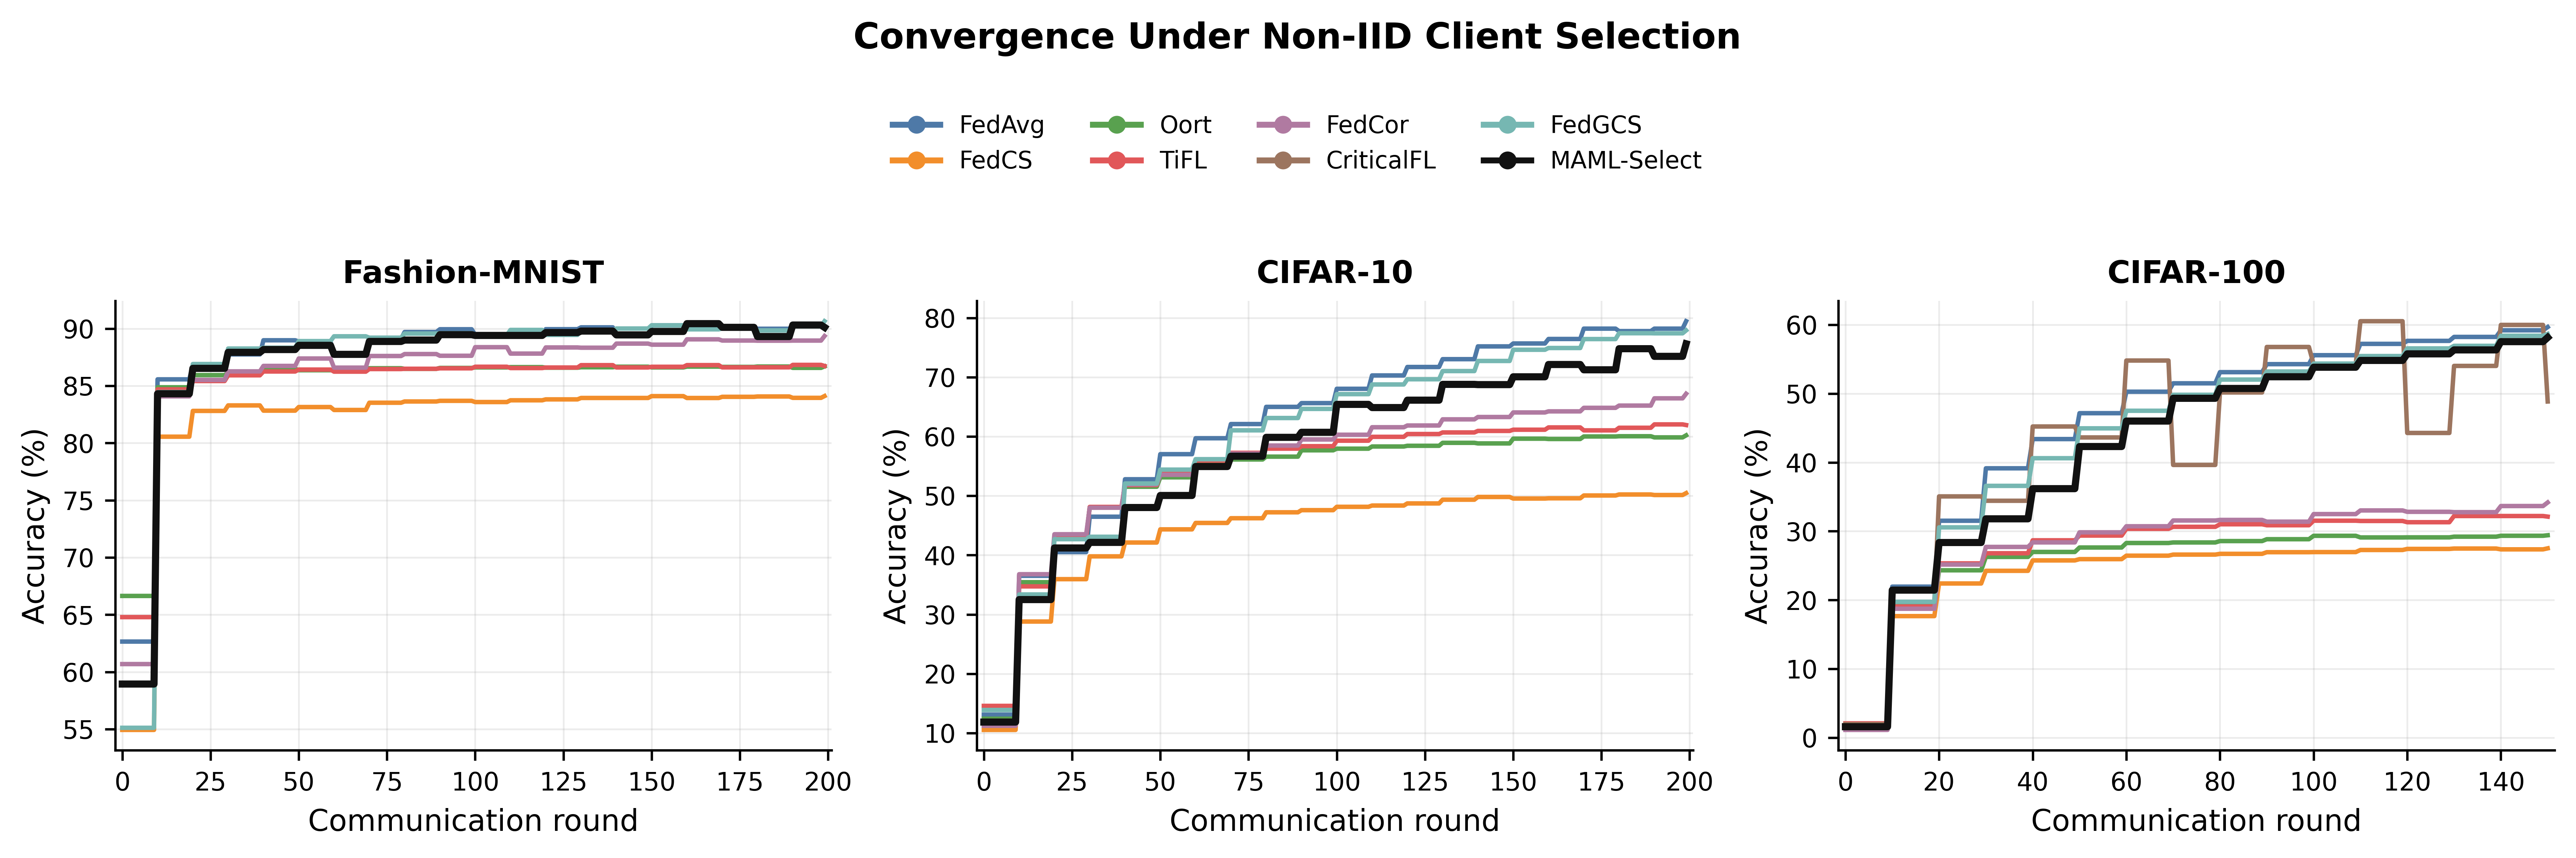
\includegraphics[width=0.94\textwidth]{review_fig_convergence_all_datasets.png}
\caption{All-dataset convergence summary used to check consistency before curating the main-letter figures. The main paper reports the final CIFAR-100 four-panel version because it is the hardest setting and includes CriticalFL.}
\label{fig:supp_convergence_all}
\end{figure}

\begin{figure}[!ht]
\centering
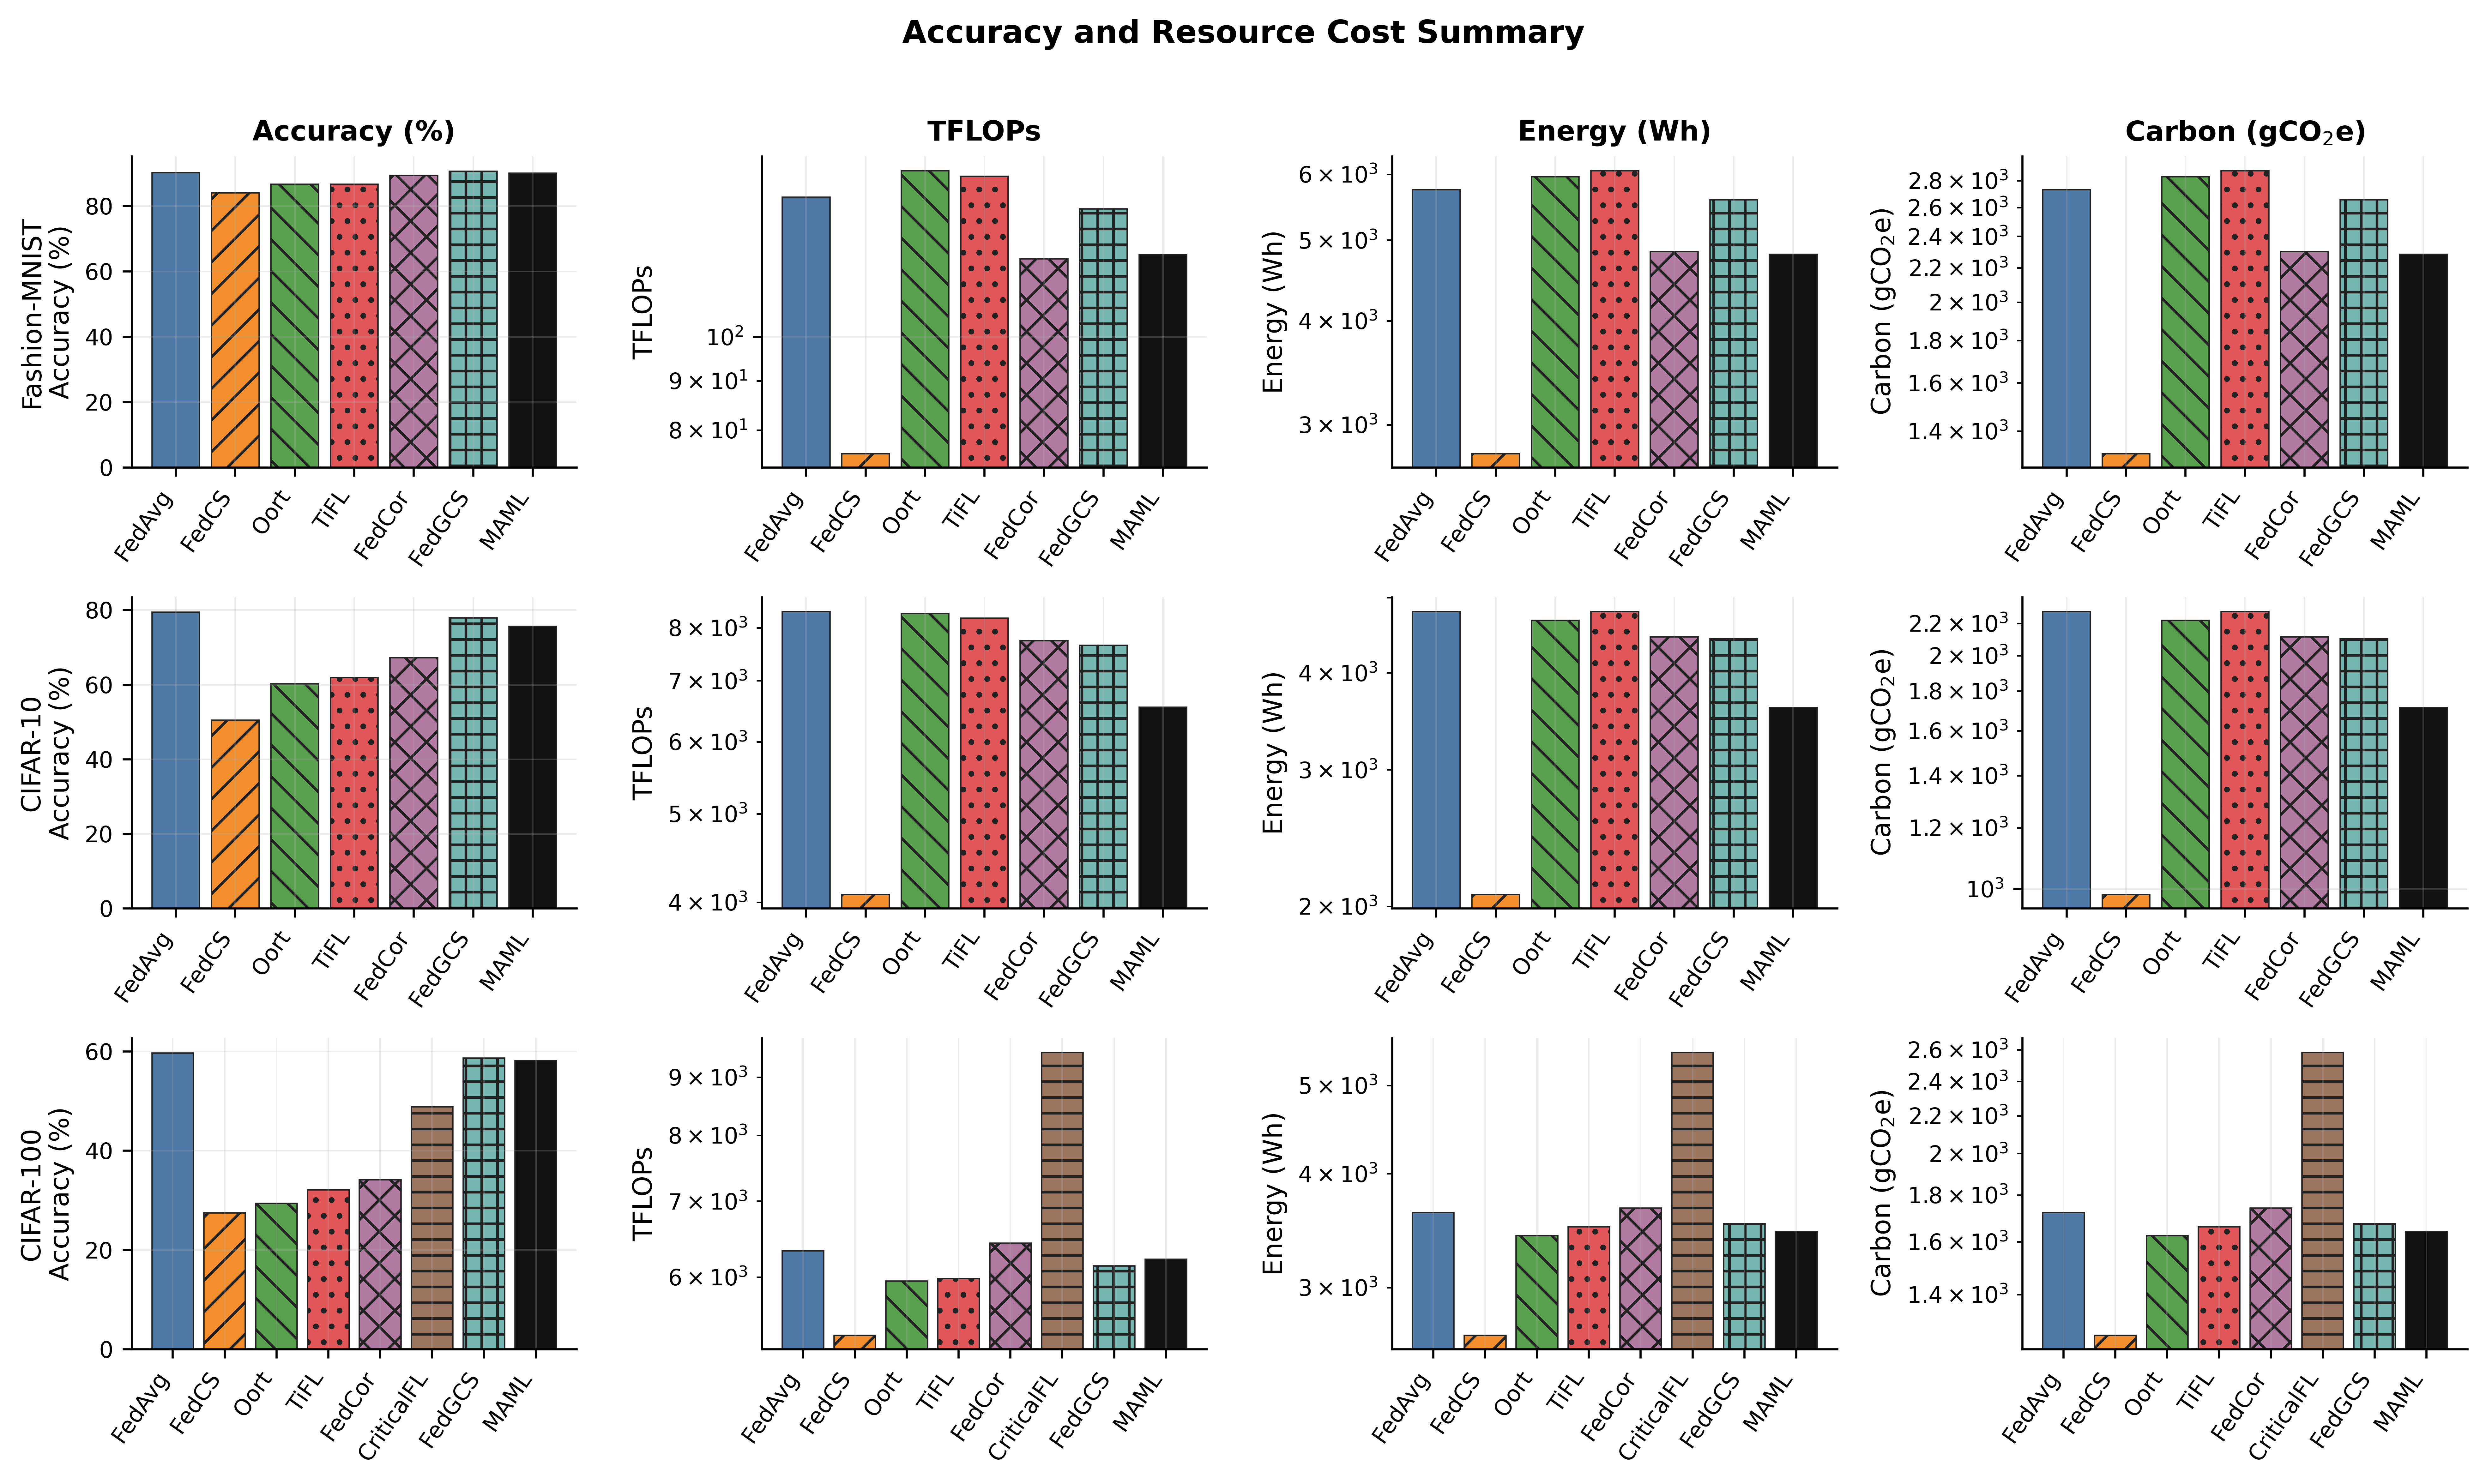
\includegraphics[width=0.96\textwidth]{review_fig_efficiency_resource_grid.png}
\caption{Expanded accuracy/resource grid across datasets and methods. This plot is retained as supplementary evidence because the main letter reports the same information more compactly through the benchmark table and trade-off figure.}
\label{fig:supp_resource_grid}
\end{figure}

\begin{figure}[!ht]
\centering
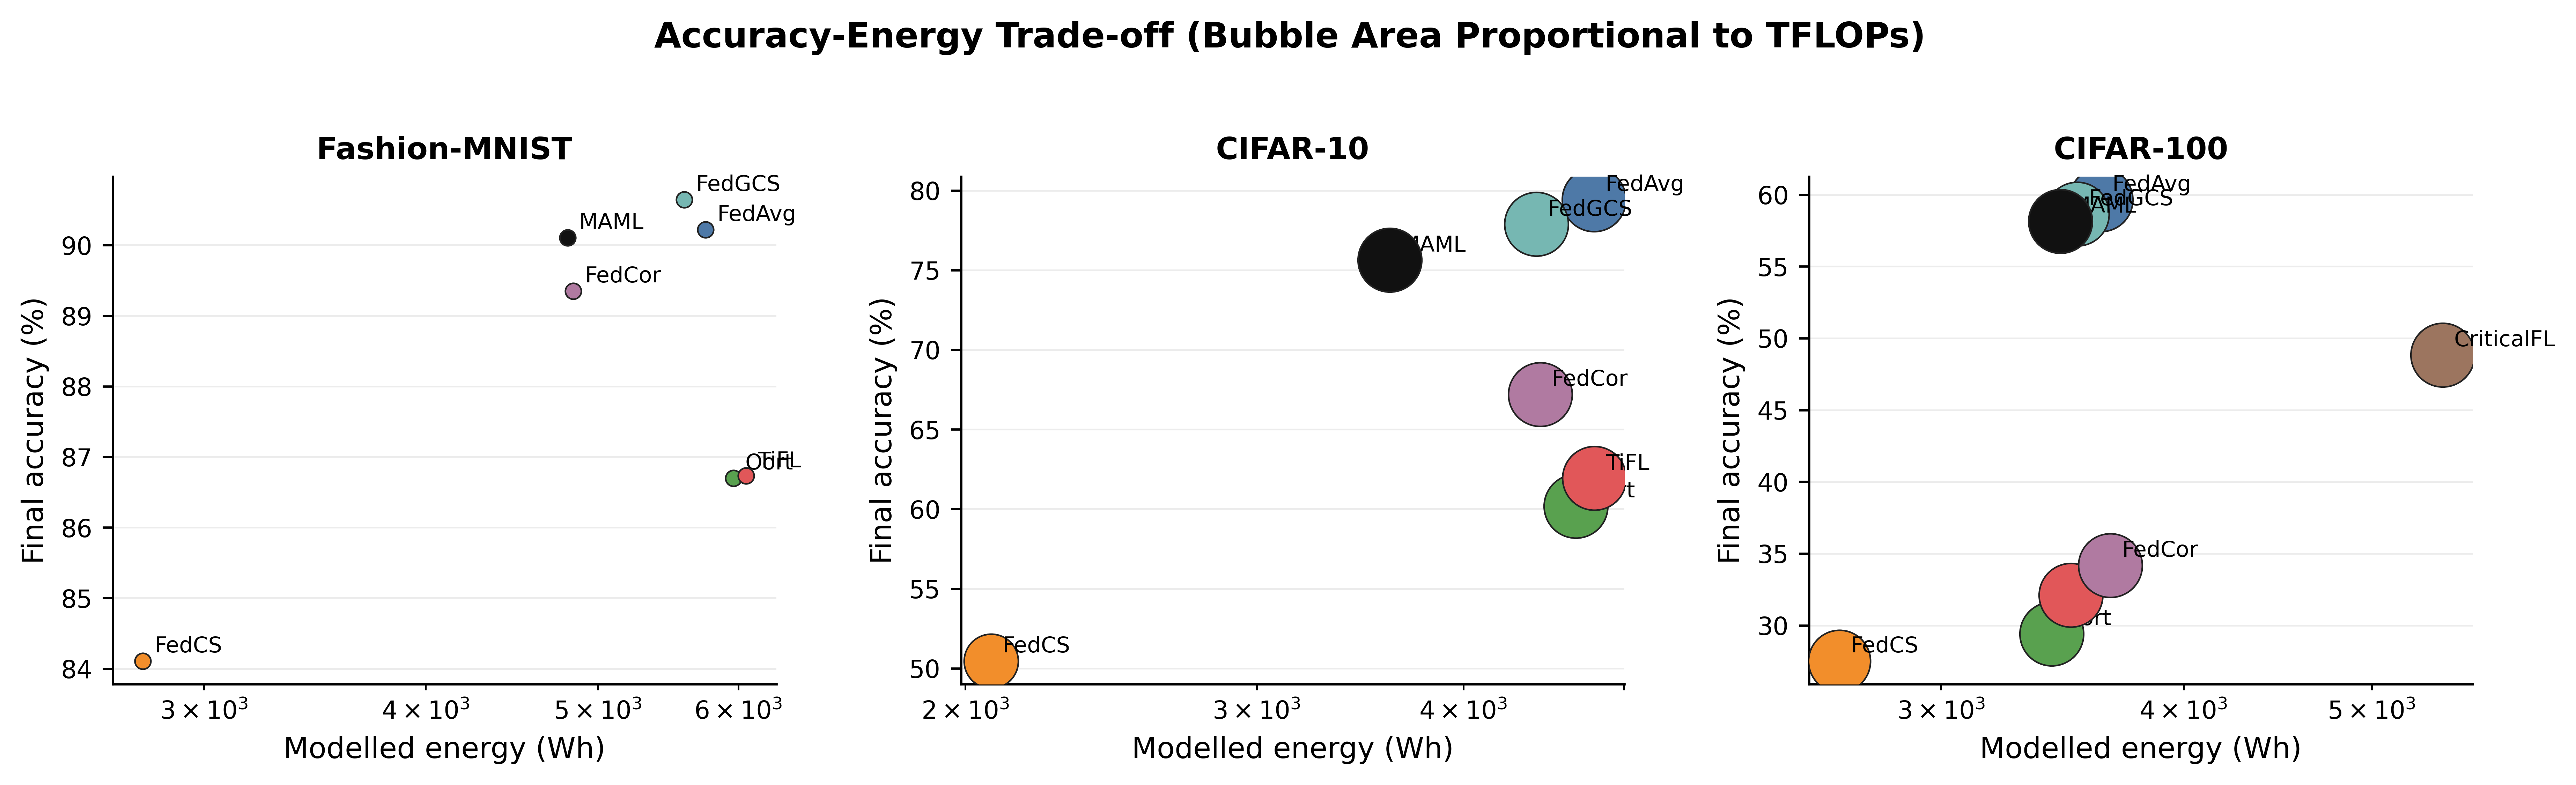
\includegraphics[width=0.74\textwidth]{review_fig_accuracy_energy_tradeoff.png}
\caption{Accuracy--energy trade-off view used as a cross-check for the final normalized trade-off plot. The main paper uses the normalized compute view because communication is identical across selectors and the TFLOP axis is easier to compare across datasets.}
\label{fig:supp_accuracy_energy}
\end{figure}

\begin{figure}[!ht]
\centering
\begin{minipage}{0.49\textwidth}
\centering

\includegraphics[width=\linewidth]{review_fig_lambda_sensitivity.png}
\caption*{(a) $\lambda$ sensitivity.}
\end{minipage}
\hfill
\begin{minipage}{0.49\textwidth}
\centering

\includegraphics[width=\linewidth]{review_fig_feature_ablation.png}
\caption*{(b) State-feature ablation.}
\end{minipage}
\caption{Design-analysis plots on Fashion-MNIST. The selected operating point is $\lambda=0.5$. Accuracy remains stable over the sweep, while larger $\lambda$ reduces compute, energy, and carbon at the cost of participation fairness.}
\label{fig:supp_lambda_ablation_side}
\end{figure}

\begin{figure}[!ht]
\centering
\begin{minipage}{0.49\textwidth}
\centering
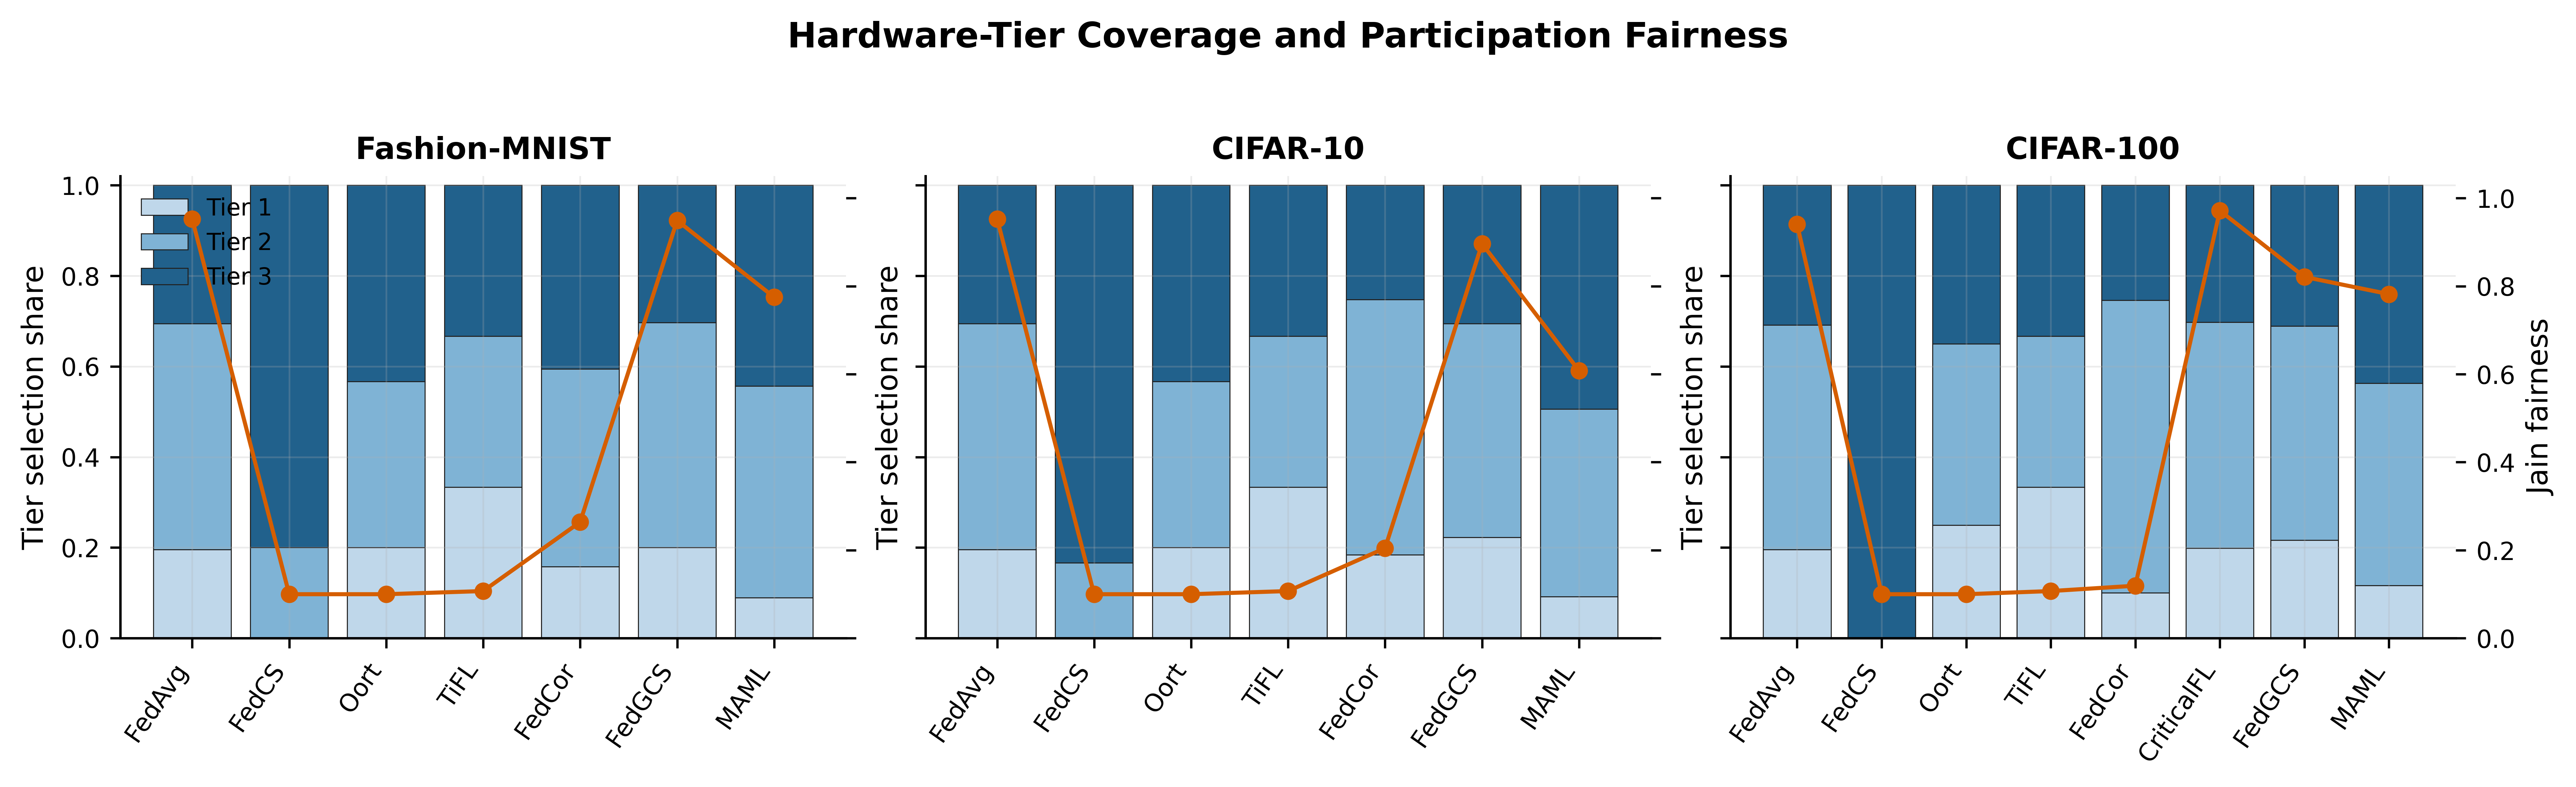
\includegraphics[width=\linewidth]{review_fig_fairness_tier_coverage.png}
\caption*{(a) Fairness and tier coverage.}
\end{minipage}
\hfill
\begin{minipage}{0.49\textwidth}
\centering
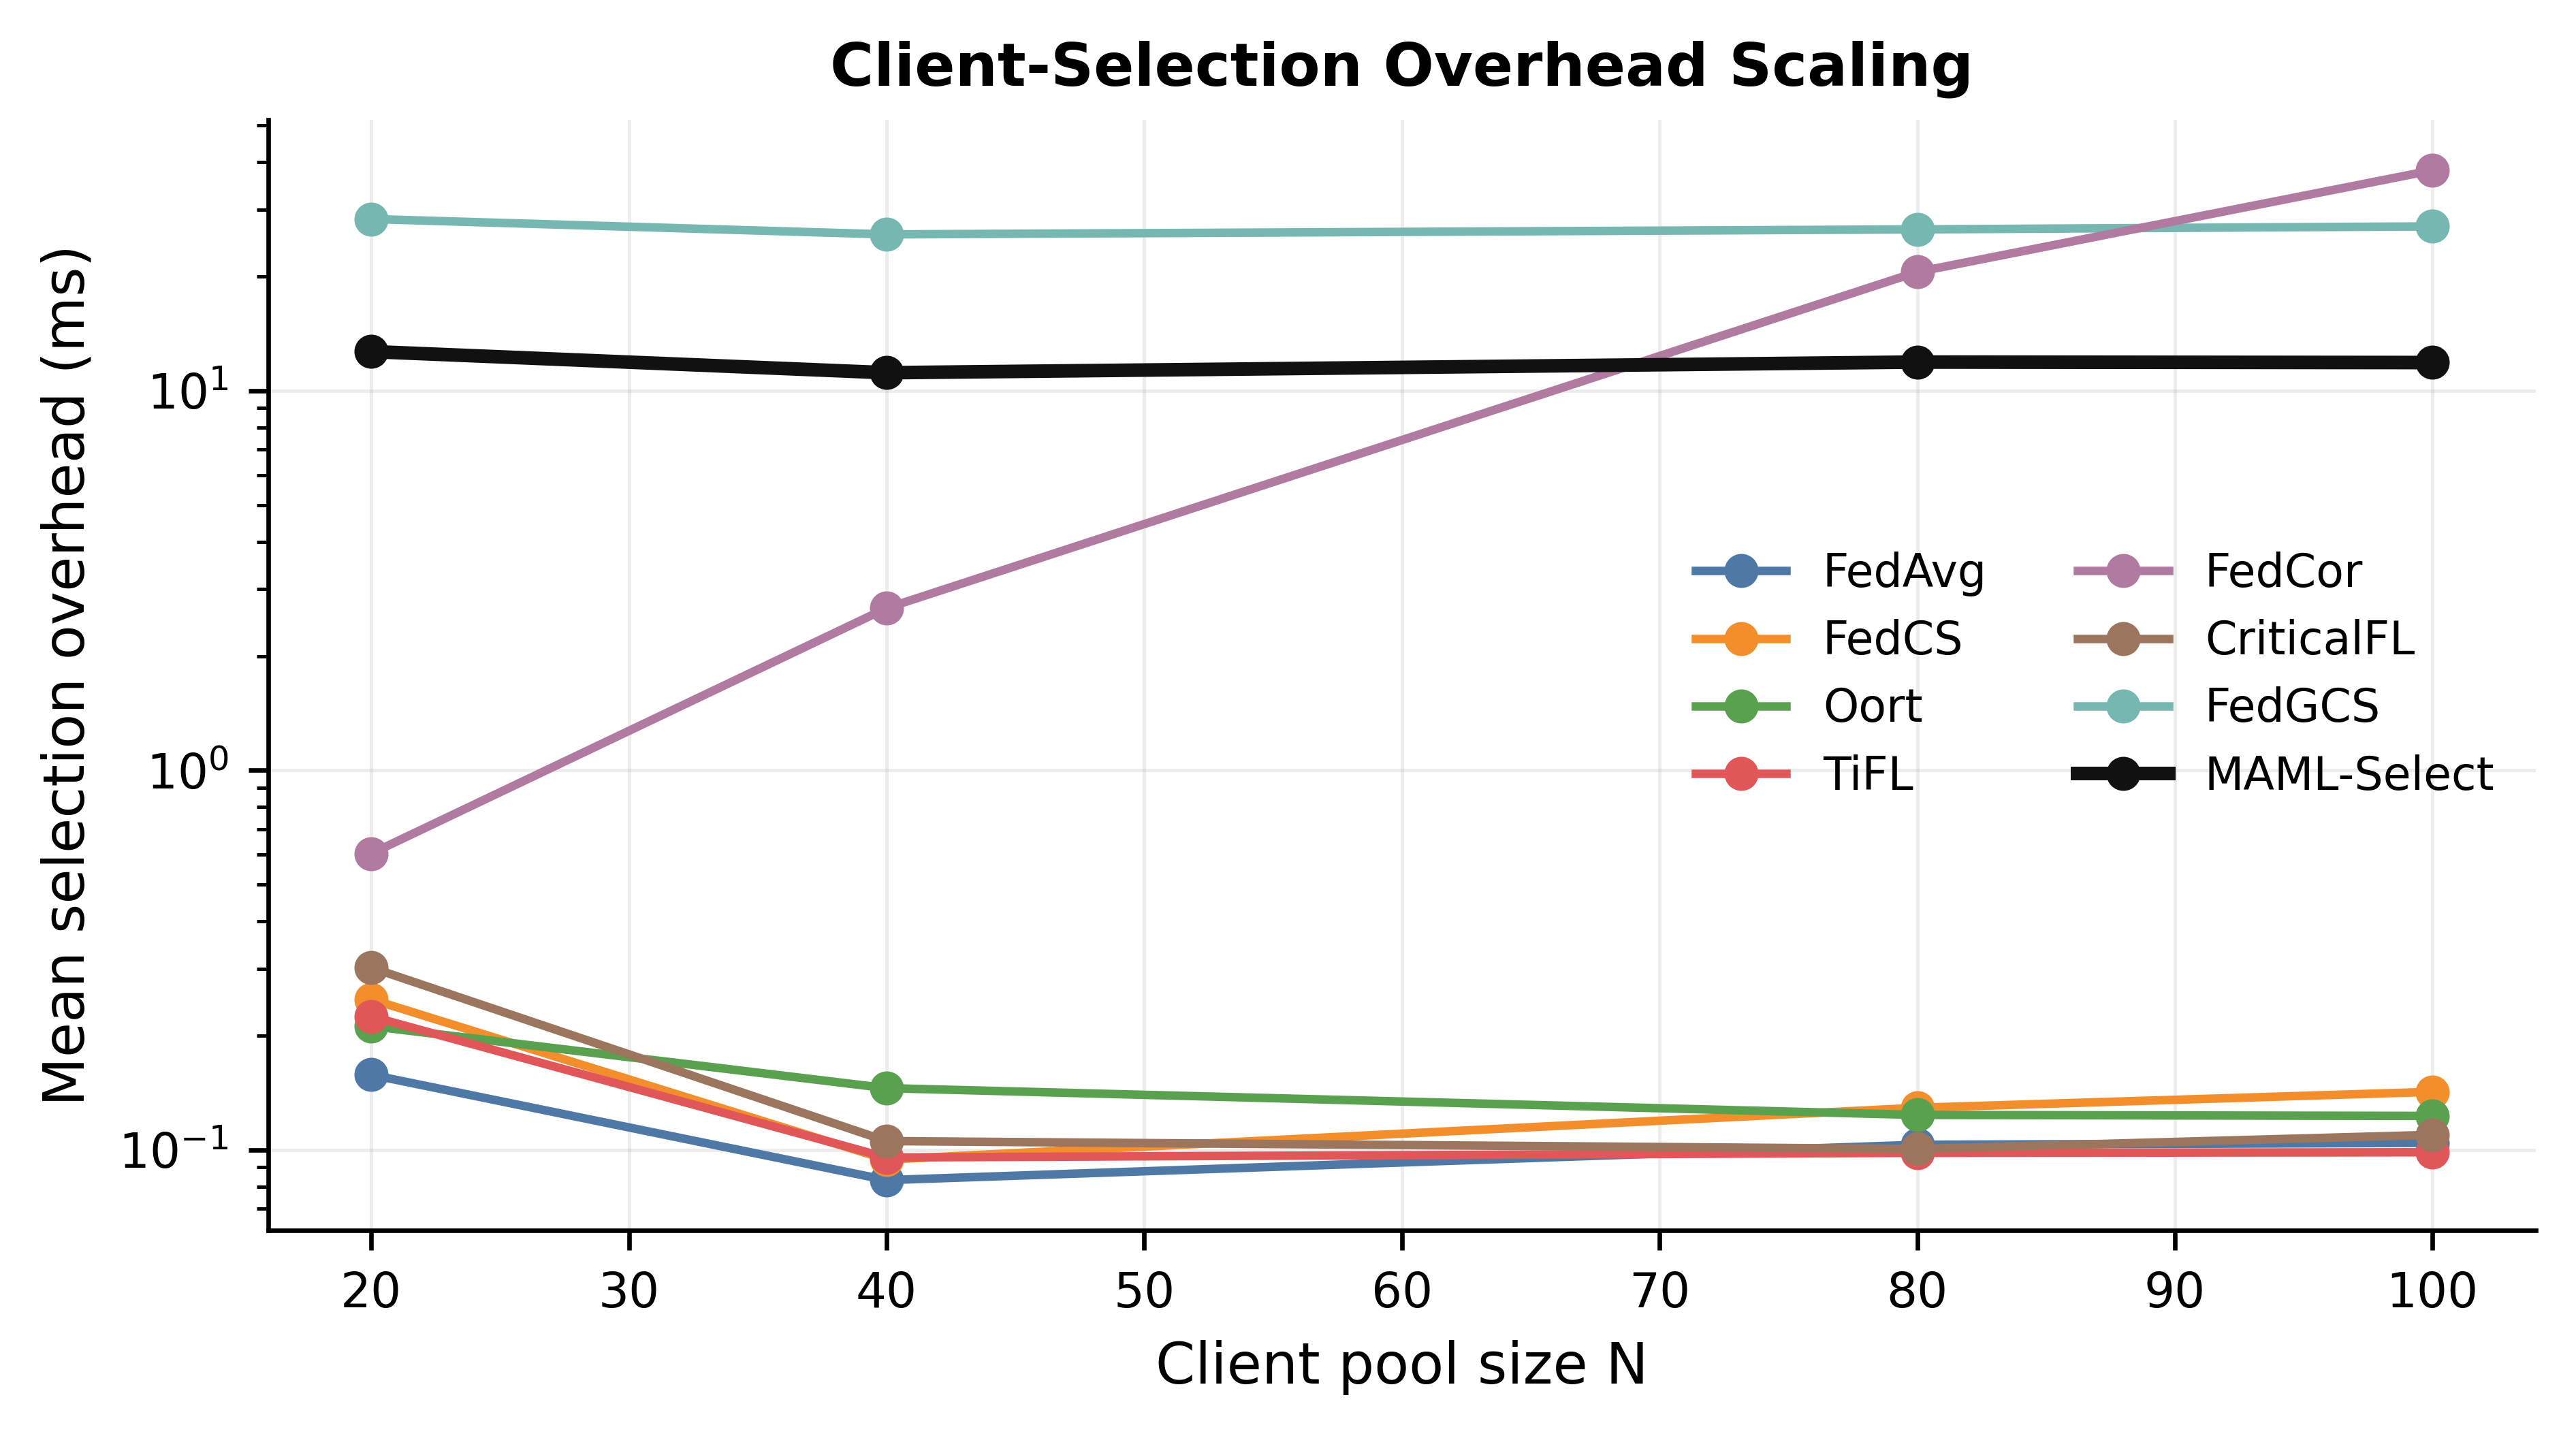
\includegraphics[width=\linewidth]{review_fig_scaling_overhead.png}
\caption*{(b) Selector overhead scaling.}
\end{minipage}
\caption{Reviewer-requested fairness and scalability checks. MAML-Select reaches full client coverage in the main runs, but its Jain index is below FedAvg and FedGCS; therefore the revised paper reports fairness transparently and does not claim fairness superiority. Selection overhead remains negligible relative to local training.}
\label{fig:supp_fairness_scaling_side}
\end{figure}

\section*{S3. MAML-Select Relative to FedAvg}

\begin{table}[!ht]
\centering
\caption{MAML-Select relative to FedAvg over shared seeds. Positive reductions indicate lower resource use for MAML-Select; $\Delta$Acc. is signed.}
\label{tab:supp_maml_vs_fedavg}
\small
\begin{tabular}{@{}lrrrrr@{}}
\toprule
Dataset & $\Delta$Acc. (pp) & TFLOPs $\downarrow$ (\%) & Energy $\downarrow$ (\%) & Carbon $\downarrow$ (\%) & $n$ \\
\midrule
Fashion-MNIST & -0.11 & 12.8 & 16.4 & 16.4 & 3 \\
CIFAR-10 & -3.81 & 21.5 & 24.7 & 24.7 & 3 \\
CIFAR-100 & -1.51 & 1.7 & 4.7 & 4.7 & 3 \\
\bottomrule
\end{tabular}
\end{table}

\begin{table}[!ht]
\centering
\caption{Paired tests for MAML-Select against FedAvg over shared seeds ($n=3$). Negative signed differences mean MAML-Select is lower than FedAvg.}
\label{tab:supp_paired_fedavg}
\small
\begin{tabular}{@{}lrrrrrrrr@{}}
\toprule
Dataset & $\Delta$Acc. & $p$ & $\Delta$TFLOPs & $p$ & $\Delta$Energy & $p$ & $\Delta$Carbon & $p$ \\
\midrule
Fashion-MNIST & -0.11 pp & 0.840 & -17.93 & 0.009 & -943.6 Wh & 0.007 & -448.2 g & 0.007 \\
CIFAR-10 & -3.81 pp & 0.041 & -1792.16 & 0.002 & -1187.4 Wh & 0.001 & -564.0 g & 0.001 \\
CIFAR-100 & -1.51 pp & 0.039 & -107.80 & 0.012 & -169.6 Wh & 0.003 & -80.6 g & 0.003 \\
\bottomrule
\end{tabular}
\end{table}

\section*{S4. Sensitivity, Ablation, and Overhead Tables}

\begin{table}[!ht]
\centering
\caption{$\lambda$ sensitivity on Fashion-MNIST ($n=3$). Accuracy is reported as mean $\pm$ s.d.; remaining columns are means.}
\label{tab:supp_lambda}
\small
\begin{tabular}{@{}lrrrrr@{}}
\toprule
$\lambda$ & Acc. (\%) & TFLOPs & Energy (Wh) & Carbon (g) & Jain \\
\midrule
0.1 & $90.40 \pm 0.22$ & 128.3 & 5176 & 2459 & 0.91 \\
0.5 & $90.23 \pm 0.55$ & 121.6 & 4799 & 2280 & 0.78 \\
1.0 & $89.74 \pm 0.79$ & 118.6 & 4639 & 2204 & 0.71 \\
5.0 & $89.37 \pm 1.02$ & 107.8 & 4140 & 1966 & 0.50 \\
\bottomrule
\end{tabular}
\end{table}

\begin{table}[!ht]
\centering
\caption{State-feature ablation on Fashion-MNIST ($n=3$). Each row removes one feature from the six-dimensional MAML-Select state vector.}
\label{tab:supp_ablation}
\small
\begin{tabular}{@{}lrrrr@{}}
\toprule
Variant & Acc. (\%) & TFLOPs & Energy (Wh) & Jain \\
\midrule
Full state vector & $90.23 \pm 0.55$ & 121.6 & 4799 & 0.78 \\
w/o loss & $90.16 \pm 0.66$ & 122.8 & 4851 & 0.79 \\
w/o gradient norm & $90.30 \pm 0.24$ & 122.4 & 4831 & 0.78 \\
w/o latency & $90.14 \pm 0.14$ & 118.9 & 4688 & 0.70 \\
w/o battery & $89.90 \pm 0.44$ & 122.2 & 4830 & 0.79 \\
w/o frequency & $90.47 \pm 0.13$ & 115.0 & 4533 & 0.65 \\
w/o staleness & $90.37 \pm 0.19$ & 122.7 & 4838 & 0.78 \\
\bottomrule
\end{tabular}
\end{table}

\begin{table}[!ht]
\centering
\caption{Mean client-selection overhead in seconds for the scaling probe (10 rounds per setting).}
\label{tab:supp_scaling}
\small
\begin{tabular}{@{}lrrrr@{}}
\toprule
Method & $N=20$ & $N=40$ & $N=80$ & $N=100$ \\
\midrule
FedAvg & 0.000158 & 0.000083 & 0.000103 & 0.000104 \\
FedCor & 0.000604 & 0.002676 & 0.020562 & 0.038099 \\
FedGCS & 0.028355 & 0.025831 & 0.026627 & 0.027116 \\
MAML-Select & 0.012689 & 0.011160 & 0.011907 & 0.011871 \\
\bottomrule
\end{tabular}
\end{table}

\section*{S5. Interpretation for the Revised Claims}

The supplementary results support three cautious claims. First, MAML-Select is not presented as a universal accuracy winner; it is competitive with FedAvg and FedGCS while reducing modelled resource use. Second, the resource estimates follow the stated simulator assumptions for device tiers and grid intensity. Third, fairness is reported explicitly: MAML-Select reaches full client coverage, but its Jain index is lower than FedAvg and FedGCS, so the manuscript avoids claiming fairness superiority.

\end{document}
